\documentclass[aspectratio=43]{beamer}
\usepackage[english]{babel}
\usepackage{amsthm}
\usepackage{mathtools}
\usepackage{physics}
\usepackage{calligra}
\usepackage{csquotes}
\usepackage{tensor}
\usepackage[thicklines]{cancel}
\usepackage{tcolorbox}
\usepackage{pstricks}
\usepackage{setspace}
\usepackage[backend=biber, bibstyle=nature, sorting=nty, citestyle=numeric-comp]{biblatex} %Custom bibliography
    \addbibresource{bib.bib} %Load references


\DeclareMathAlphabet{\mathcalligra}{T1}{calligra}{m}{n}
\DeclareFontShape{T1}{calligra}{m}{n}{<->s*[2.2]callig15}{}
\newcommand{\scriptr}{\mathcalligra{r}\,}
\newcommand{\boldscriptr}{\pmb{\mathcalligra{r}}\,}
\def\rc{\scriptr}
\def\brc{\boldscriptr}
\def\hrc{\hat\brc}
\newcommand{\ie}{\emph{i.e.}} %id est
\newcommand{\eg}{\emph{e.g.}} %exempli gratia
\newcommand{\rtd}[1]{\ensuremath{\left\lfloor #1 \right\rfloor}}
\newcommand{\dirac}[1]{\ensuremath{\delta \left( #1 \right)}}
\newcommand{\diract}[1]{\ensuremath{\delta^3 \left( #1 \right)}}
\newcommand{\e}{\ensuremath{\epsilon_0}}
\newcommand{\m}{\ensuremath{\mu_0}}
\newcommand{\V}{\ensuremath{\mathcal{V}}}
\newcommand{\prnt}[1]{\ensuremath{\left(#1\right)}} %parentheses
\newcommand{\colch}[1]{\ensuremath{\left[#1\right]}} %square brackets
\newcommand{\chave}[1]{\ensuremath{\left\{#1\right\}}}  %curly brackets

\useoutertheme{infolines}
\useinnertheme{rectangles}
\usefonttheme{professionalfonts}


\definecolor{orange}{HTML}{f28165}
\definecolor{gray}{HTML}{303030}
\definecolor{yellow}{HTML}{f0be52}
\definecolor{lightorange}{HTML}{f19e58}

\renewcommand{\CancelColor}{\color{orange}}

\makeatletter
\newcommand{\mybox}[1]{%
  \setbox0=\hbox{#1}%
  \setlength{\@tempdima}{\dimexpr\wd0+13pt}%
  \begin{tcolorbox}[colback=orange,colframe=orange,boxrule=0.5pt,arc=4pt,
      left=6pt,right=6pt,top=6pt,bottom=6pt,boxsep=0pt,width=\@tempdima]
    \textcolor{white}{#1}
  \end{tcolorbox}
}
\makeatother

\usecolortheme[named=orange]{structure}
\usecolortheme{sidebartab}
\usecolortheme{orchid}
\usecolortheme{whale}
\setbeamercolor{alerted text}{fg=yellow}
\setbeamercolor{block title alerted}{bg=alerted text.fg!90!black}
\setbeamercolor{block title example}{bg=lightorange!60!black}
\setbeamercolor{background canvas}{bg=gray}
\setbeamercolor{normal text}{bg=gray,fg=white}

\setbeamertemplate{footline}
        {
      \leavevmode%
      \hbox{%
      \begin{beamercolorbox}[wd=.25\paperwidth,ht=2.25ex,dp=1ex,center]{author in head/foot}%
        \usebeamerfont{author in head/foot}\insertshortauthor~~(\insertshortinstitute)
      \end{beamercolorbox}%
      \begin{beamercolorbox}[wd=.25\paperwidth,ht=2.25ex,dp=1ex,center]{title in head/foot}%
        \usebeamerfont{title in head/foot}\insertshorttitle
      \end{beamercolorbox}%
      \begin{beamercolorbox}[wd=.25\paperwidth,ht=2.25ex,dp=1ex,center]{date in head/foot}%
        \usebeamerfont{date in head/foot}\insertshortdate{}%\hspace*{2em}

    %#turning the next line into a comment, erases the frame numbers
        % \insertframenumber{} / \inserttotalframenumber
        % \hspace*{2ex}

      \end{beamercolorbox}

      \begin{beamercolorbox}[wd=.25\paperwidth,ht=2.25ex,dp=1ex,center]{date in head/foot}%
        % \usebeamerfont{date in head/foot}\insertshortdate{}%\hspace*{2em}
        %
      %#turning the next line into a comment, erases the frame numbers
        \insertframenumber{} / \inserttotalframenumber
        % \hspace*{2ex}
      \end{beamercolorbox}}%
      \vskip0pt%
    }


\setbeamertemplate{blocks}[rectangle]
\setbeamercovered{dynamic}

\setbeamertemplate{section page}
{
	\begin{centering}
		\begin{beamercolorbox}[sep=27pt,center]{part title}
			\usebeamerfont{section title}\insertsection\par
			\usebeamerfont{subsection title}\insertsubsection\par
		\end{beamercolorbox}
	\end{centering}
}

%\setbeamertemplate{subsection page}
%{
%	\begin{centering}
%		\begin{beamercolorbox}[sep=12pt,center]{part title}
%			\usebeamerfont{subsection title}\insertsubsection\par
%		\end{beamercolorbox}
%	\end{centering}
%}

\newcommand{\hlight}[1]{\colorbox{violet!50}{#1}}
\newcommand{\hlighta}[1]{\colorbox{red!50}{#1}}

\title{Introduction to} %->->->->-> Check hyperref title <-<-<-<-<-
\subtitle{Optimization Method}
\author[Li]{Li\cdot Zikang}
\institute[USTC]{
    School of Management%
    \\%
    University of Science and Technology of China %
} %You can change the Institution if you are from somewhere else
\date{Sept 5, 2020}

\begin{document}

    \frame{\titlepage}
    \begin{frame}{Table of contents}
        \tableofcontents
    \end{frame}

    \section{Dynamic Programming}

    \frame{\sectionpage}

    \begin{frame}{0-1 Knapsack Problem}
        The most common problem being solved is the 0-1 knapsack problem, which restricts the number $ x_{i} $ of copies of each kind of item to zero or one. Given a set of $ n $ items numbered from 1 up to $ n $, each with a weight $ w_{i} $ and a value $ v_{i} $, along with a maximum weight capacity $ W $,
        \uncover<+->{\begin{equation*}
            \begin{align}
              \max& \sum _{i=1}^{n}v_{i}x_{i} \\
              \text{s.t.}& \sum _{i=1}^{n}w_{i}x_{i}\leq W $ \text{and} $ x_{i}\in \{0,1\}.
            \end{align}
            \end{equation*}}
    \end{frame}

    \begin{frame}{0-1 Knapsack Problem}
      \uncover<+>{Assume $ w_{1},\,w_{2},\,\ldots ,\,w_{n},\,W $ are strictly positive integers. Define $ m[i,w] $ to be the maximum value that can be attained with weight less than or equal to $ w $ using items up to $ i $.
      We can define $ m[i,w] $ recursively as follows:}
        \uncover<+>{\begin{equation*}
          $ m[0,\,w]=0 $
        \end{equation*}
        \begin{equation*}
          $ m[i,\,w]=m[i-1,\,w] $ if $ w_{i}>w\,\! $
        \end{equation*}
        \begin{equation*}
          $ m[i,\,w]=\max(m[i-1,\,w],\,m[i-1,w-w_{i}]+v_{i}) $ if $ w_{i}\leqslant w $.
        \end{equation*}}
    \end{frame}

    \begin{frame}{0-1 Knapsack Problem}
      \uncover<+->{The solution can then be found by calculating $ m[n,W] $. To do this efficiently, we can use a table to store previous computations.
      This solution will therefore run in $ O(nW) $ time and $ O(nW) $ space.}\\

      \centering
      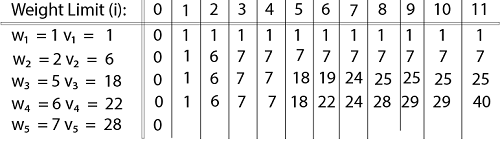
\includegraphics[width = 0.8\textwidth]{images/0-1-knapsack-problem1.png}
    \end{frame}

    \begin{frame}{Optimal substructure}
      \begin{itemize}
        \justifying
        \item Fibonacci sequence
        \begin{equation*}
          fib(n) = fib(n-1) + fib(n-2)
        \end{equation*}
        \item Dijkstra's algorithm for the shortest path problem
        \begin{equation*}
          d[y] = \min_x\{d[y], d[x]+w(x,y)\}
        \end{equation*}
      \end{itemize}
      How to define the status and stage of problems is essential.
    \end{frame}

    \begin{frame}{Shortest path problem}
        Given a directed graph $(V, A)$ with source node $s$, target node $t$, and cost $w_{ij}$  for each edge $(i, j)$ in $A$, consider the program with variables $x_{ij}$.
        \centering
        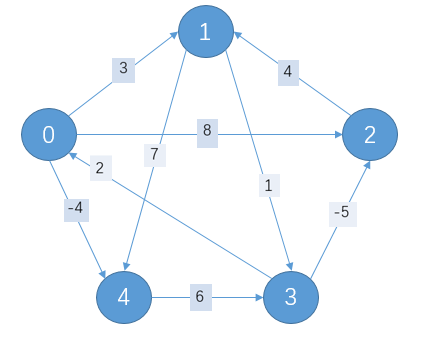
\includegraphics[width = 0.6\textwidth]{images/Shortest1.png}
    \end{frame}

    \begin{frame}{Shortest path problem}
      \begin{itemize}
        \item Integer programming formulation:
      \end{itemize}
      \begin{equation*}
        \begin{align}
        \min& \sum_{(i,j)\in A}w_{ij}x_{ij}\\
        \text{s.t.} &\sum_{j}x_{ij}-\sum_{j}x_{ji}={\begin{cases}1,&{\text{if }}i=s;\\-1,&{\text{if }}i=t;\\0,&{\text{ otherwise.}}\end{cases}}\\
        & x\in \{0,1\} ~\text{and for all} ~i.
        \end{align}
      \end{equation*}
    \end{frame}

    \begin{frame}{Shortest path problem}
      \begin{itemize}
        \item Find the shortest path from s to t.
        \centering
        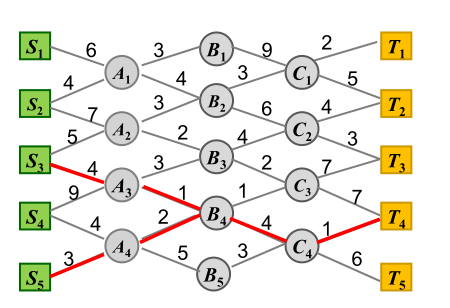
\includegraphics[width = 0.8\textwidth]{images/Shortest3.png}
      \end{itemize}
    \end{frame}

    \begin{frame}{Shortest path problem}
    \begin{equation*}
      \begin{align}
    \textcolor{yellow}{Stage 1}\quad &F(C_l) = \min_m\{C_lT_m\} \\
    \vspace{4pt}
    \textcolor{red}{Stage 2}\quad &F(B_k) = \min_l\{B_kC_l+F(C_l)\} \\
    \vspace{4pt}
    \textcolor{blue}{Stage 3}\quad &F(A_j) = \min_k\{A_jB_k+F(B_k)\} \\
    \vspace{4pt}
    \textcolor{green}{Stage 4}\quad &F(S_i) = \min_j\{S_iA_j+F(A_j)\}
    \end{align}
    \end{equation*}
    \end{frame}

    \begin{frame}{Shortest path problem}
      \begin{itemize}
        \item Find the shortest path from s to t.
        \centering
        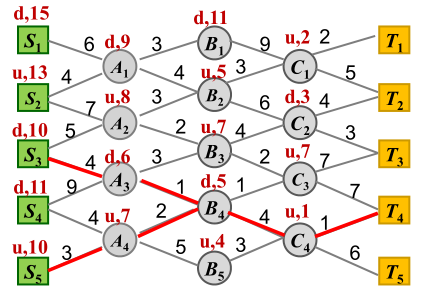
\includegraphics[width = 0.8\textwidth]{images/Shortest2.png}
      \end{itemize}
    \end{frame}
 %You can put the frames directly into the presentation, but using the input command and writing them in separate .tex files might be more organized

    \section{Integer \& Linear Programming}

    \frame{\sectionpage}
    %
    % $ {\displaystyle {\text{maximize}}~~\sum _{(i,j)\in A\times T}w_{ij}x_{ij}} $
    % $ {\displaystyle {\text{subject to}}~~\sum _{j\in T}x_{ij}=1{\text{ for }}i\in A,\,~~~\sum _{i\in A}x_{ij}=1{\text{ for }}j\in T} $
    % $ {\displaystyle 0\leq x_{ij}\leq 1{\text{ for }}i,j\in A,T,\,} $
    % $ {\displaystyle x_{ij}\in \mathbb {Z} {\text{ for }}i,j\in A,T.} $

    \begin{frame}{Integer Programming}
        \begin{itemize}
          \item Shortest path problem
          \begin{equation*}
            \begin{align}
            \min& \sum_{(i,j)\in A}w_{ij}x_{ij}\\
            \text{s.t.} &\sum_{j}x_{ij}-\sum_{j}x_{ji}={\begin{cases}1,&{\text{if }}i=s;\\-1,&{\text{if }}i=t;\\0,&{\text{ otherwise.}}\end{cases}}\\
            & x\in \{0,1\} ~\text{and for all} ~i.
            \end{align}
          \end{equation*}
          \item<+-> Maximum flow problem
          \item<+-> Assignment problem
        \end{itemize}
    \end{frame}

    \begin{frame}{Totally Unimodular Matrix}
      \begin{itemize}
        \item Every entry in A is 0, +1, or −1;
        \item Every column of A contains at most two non-zero (i.e., +1 or −1) entries;
        \item If two non-zero entries in a column of A have the same sign, then the row of one is in B, and the other in C;
        \item If two non-zero entries in a column of A have opposite signs, then the rows of both are in B, or both in C.
      \end{itemize}
    \end{frame}

    \begin{frame}{TU Matrix}
      \begin{itemize}
        \item Totally unimodular matrices are extremely important in polyhedral combinatorics and combinatorial optimization since they give a quick way to verify that a linear program is integral (has an integral optimum, when any optimum exists).
        \item Specifically, if A is TU and b is integral, then linear programs of forms like $ \{\min cx\mid Ax\geq b,x\geq 0\} $ or $ \{\max cx\mid Ax\leq b\} $ have integral optima, for any c. Hence if A is totally unimodular and b is integral, every extreme point of the feasible region (e.g. $ \{x\mid Ax\geq b\} $) is integral and thus the feasible region is an integral polyhedron.
      \end{itemize}
    \end{frame}

    \begin{frame}{Another Perspective}
      Recall the simplex method for linear programming.
      \begin{equation*}
        \begin{align}
        Bx &= b \\
        x^* &= (B^{-1}b,0) \\
        \end{align}
      \end{equation*}
      How to obtain the inverse of B?

      Cramer's rule: \[B^{-1} = B^*/\text{det}(B)\]
    \end{frame}

    \begin{frame}{Simplex Method}
      \begin{itemize}
        \item Feasible region(Convex polytope)
        \item Basic feasible solution(Extreme point)
        \item Basic variables(Identity matrix)
        \item Entering variable selection
        \item Leaving variable selection
        \item Pivot operation
        \item Reduced costs
      \end{itemize}
    \end{frame}

    \begin{frame}{Another Perspective}
      The simplex method is an iteration process.
      \begin{equation*}
        \begin{align}
        x' = x – \theta\lambda
        \end{align}
      \end{equation*}
      How to obtain the inverse of B?
      \begin{block}
        {Cramer's rule:}
        {\centering\[B^{-1} = B^*/\text{det}(B)\]}
      \end{block}
    \end{frame}


    \section{General Optimization Methods}

    \begin{frame}{General Optimization Methods}
        \centering
        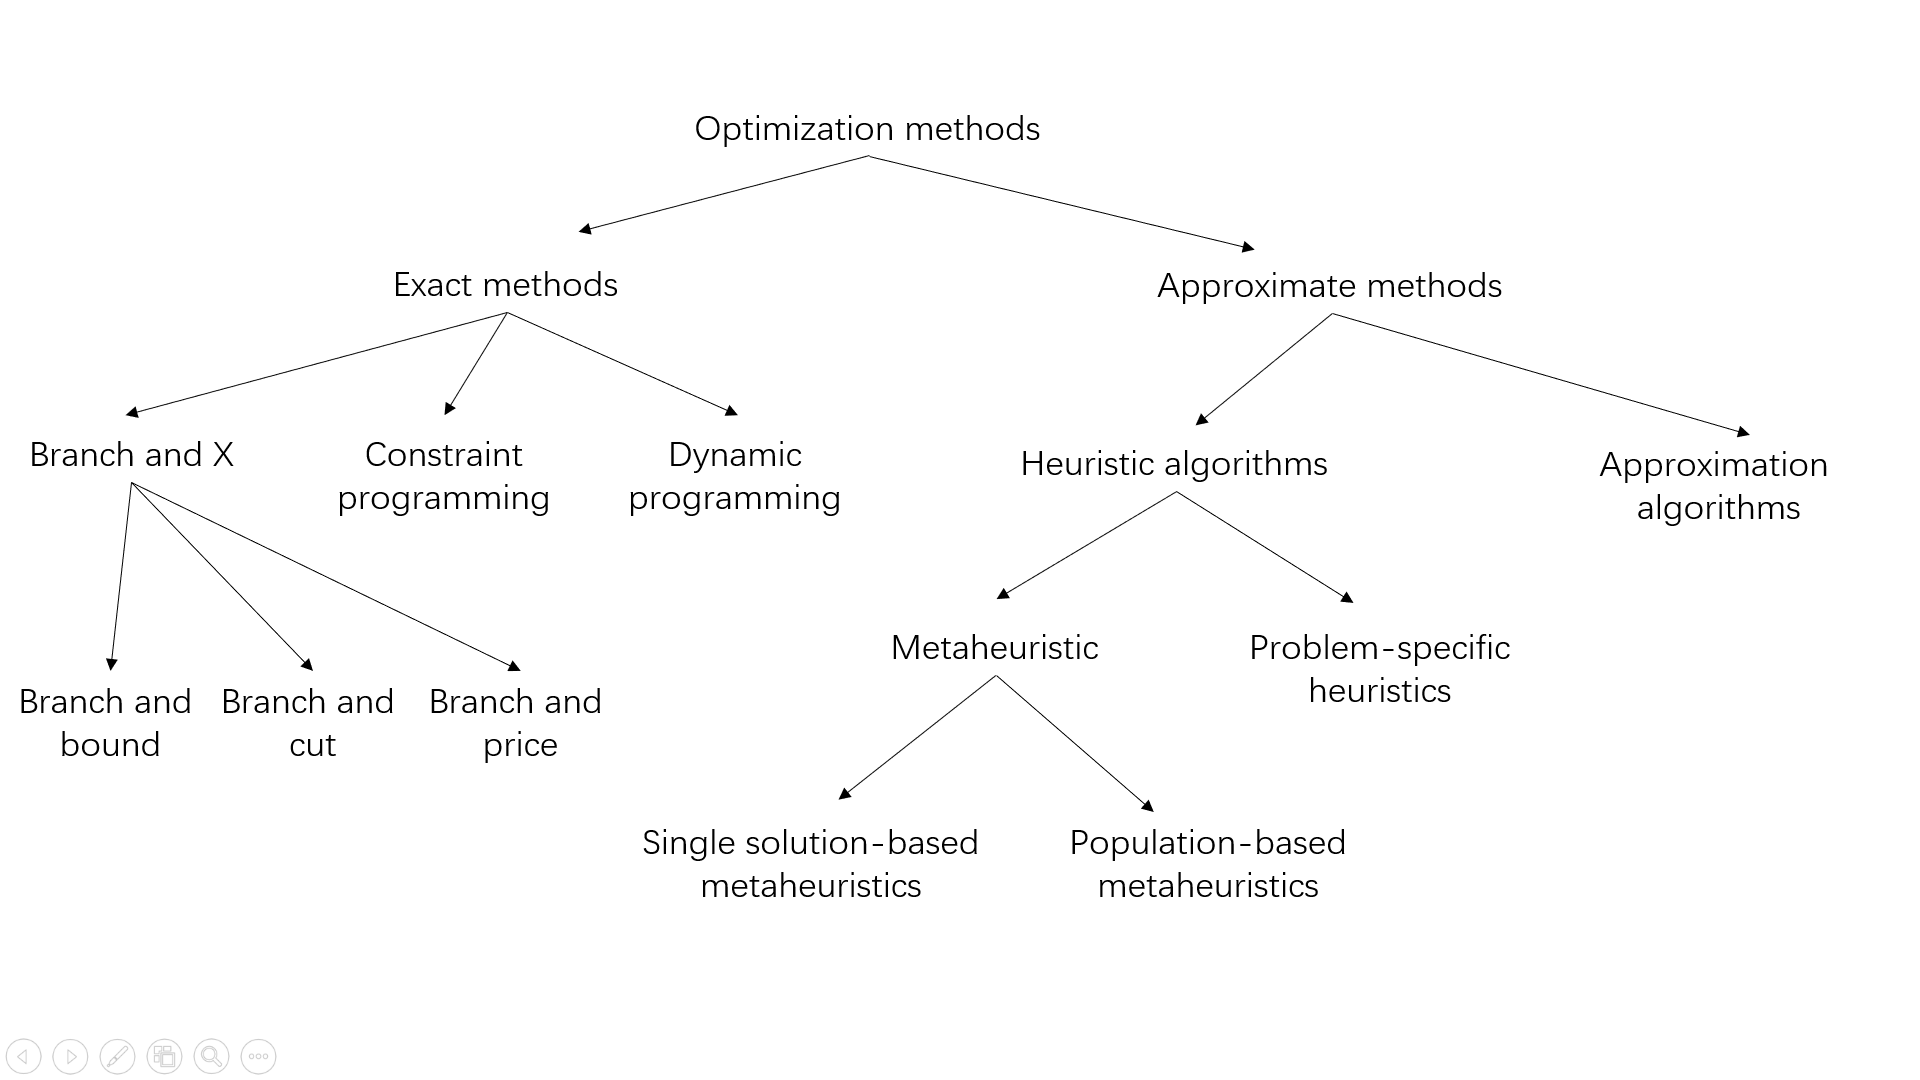
\includegraphics[width = 1\textwidth]{images/opt.png}
    \end{frame}

    \subsection{Exact Methods}
    \frame{\sectionpage}

    \begin{frame}{Exact Methods}
      \begin{itemize}
        \item<+-> Branch and X
          \begin{enumerate}
          \item<+>  Branch and bound
          \item<+>  Branch and cut
          \item<+>  Branch and price
          \end{enumerate}
      \end{itemize}
    \end{frame}

    \begin{frame}{Branch and bound}
      \centering
      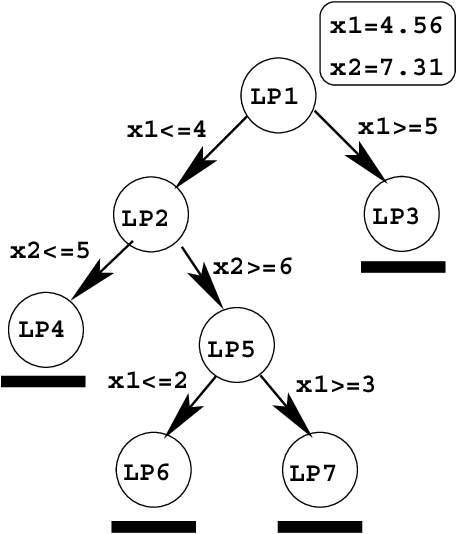
\includegraphics[width = 0.55\textwidth]{images/Branch.png}
    \end{frame}

    \begin{frame}{Cutting Plane Method}
      \centering
      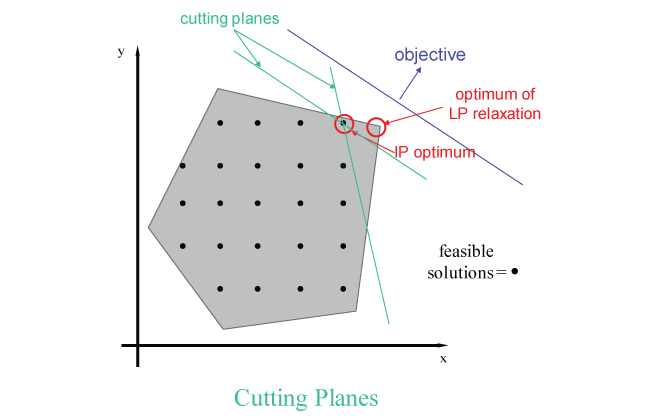
\includegraphics[width = 1\textwidth]{images/CP.png}
    \end{frame}

    \begin{frame}{Gomory's Cut}
      \begin{itemize}

      \item Using the simplex method:
      $x_{i}+\sum{\bar {a}}_{i,j}x_{j}={\bar {b}}_{i}$ \\

      where $x_i$ are the basic variables and the $x_j$'s are the nonbasic variables.

      \item Rewrite this equation: integer parts(left) and the fractional parts(right):

      $x_{i}+\sum \lfloor {\bar {a}}_{i,j}\rfloor x_{j}-\lfloor {\bar {b}}_{i}\rfloor ={\bar {b}}_{i}-\lfloor {\bar {b}}_{i}\rfloor -\sum ({\bar {a}}_{i,j}-\lfloor {\bar {a}}_{i,j}\rfloor )x_{j}.$ \\

      \item Right side is less than 1 and the left side is an integer, therefore the inequality:
      \textcolor{red}{${\bar {b}}_{i}-\lfloor {\bar {b}}_{i}\rfloor -\sum ({\bar {a}}_{i,j}-\lfloor {\bar {a}}_{i,j}\rfloor )x_{j}\leq 0 $}
      must hold for any integer point in the feasible region.

      \item The inequality above is a cut with the desired properties. Introducing a new slack variable $x_k$ for this inequality, a new constraint is added to the linear program, namely

      \textcolor{red}{$x_{k}+\sum (\lfloor {\bar {a}}_{i,j}\rfloor -{\bar {a}}_{i,j})x_{j}=\lfloor {\bar {b}}_{i}\rfloor -{\bar {b}}_{i},\,x_{k}\geq 0,\,x_{k}{\mbox{ an integer}}$.}
      \end{itemize}
    \end{frame}

    \begin{frame}{Branch and price}
      \centering
      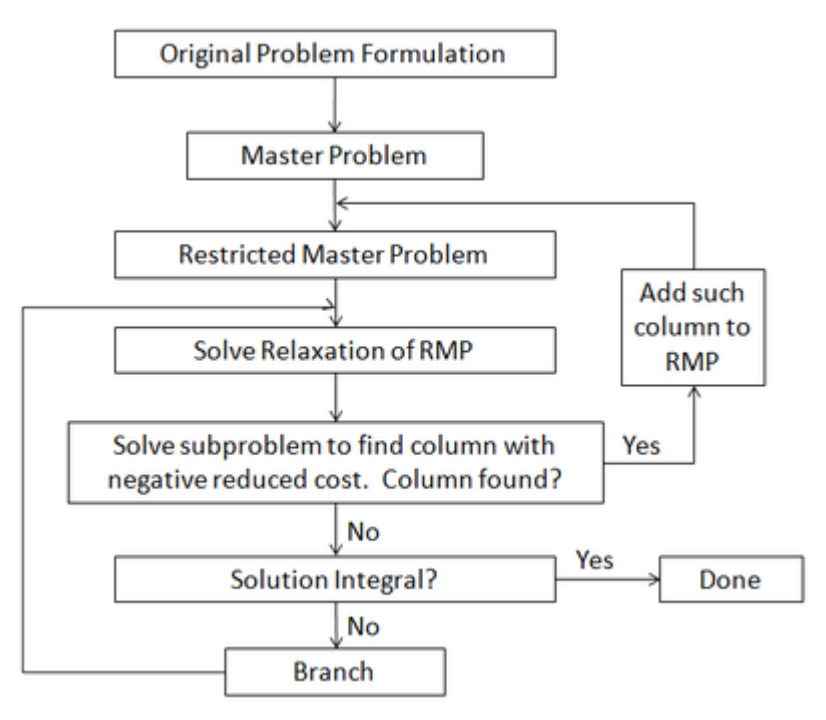
\includegraphics[width = 0.7\textwidth]{images/branch_price.png}
    \end{frame}

    \begin{frame}{Exact Methods}
      \begin{itemize}
        \item Branch and X
        \item<+-> Dynamic programming
        \item<+-> Constraint programming
        \item<+-> Enumeration method
      \end{itemize}
    \end{frame}



    \subsection{Approximate Methods}
    \frame{\sectionpage}

    \begin{frame}{Approximate Methods}
      \begin{itemize}
        \item Heuristic algorithms
        \vspace{4pt}
        \begin{enumerate}
          \item<+->  Metaheuristic
            \begin{enumerate}
              \item<+>[*] Single solution-based metaheuristics
              \item<+>[*] Population-based metaheuristics
            \end{enumerate}
          \vspace{4pt}
          \item<+->  Problem-specific heuristics
        \end{enumerate}
        \vspace{10pt}
        \item<+-> Approximate algorithms
      \end{itemize}
    \end{frame}

    \begin{frame}{Single solution-based metaheuristics}
      \begin{itemize}
        \item Simulated Annealing Algorithm
        \item Tabu Search
        \item Variable Neighborhood Search
        \item Adaptive Large Neighborhood Search
      \end{itemize}
    \end{frame}

    \begin{frame}{Population-based heuristics}
      \begin{itemize}
        \item Genetic Algorithm
        \item Ant Colony Optimization
        \item Partical Swarm Optimization
      \end{itemize}
    \end{frame}

    % Using the simplex method to solve a linear program produces a set of equations of the form
    % $x_{i}+\sum{\bar {a}}_{i,j}x_{j}={\bar {b}}_{i}$ \\
    %
    % where xi is a basic variable and the xj's are the nonbasic variables. Rewrite this equation so that the integer parts are on the left side and the fractional parts are on the right side:
    %
    % $x_{i}+\sum \lfloor {\bar {a}}_{i,j}\rfloor x_{j}-\lfloor {\bar {b}}_{i}\rfloor ={\bar {b}}_{i}-\lfloor {\bar {b}}_{i}\rfloor -\sum ({\bar {a}}_{i,j}-\lfloor {\bar {a}}_{i,j}\rfloor )x_{j}.$ \\
    %
    % For any integer point in the feasible region the right side of this equation is less than 1 and the left side is an integer, therefore the common value must be less than or equal to 0. So the inequality
    %
    % $ {\bar {b}}_{i}-\lfloor {\bar {b}}_{i}\rfloor -\sum ({\bar {a}}_{i,j}-\lfloor {\bar {a}}_{i,j}\rfloor )x_{j}\leq 0 $
    %
    % must hold for any integer point in the feasible region. Furthermore, nonbasic variables are equal to 0s in any basic solution and if xi is not an integer for the basic solution x,
    %
    % $ {\bar {b}}_{i}-\lfloor {\bar {b}}_{i}\rfloor -\sum ({\bar {a}}_{i,j}-\lfloor {\bar {a}}_{i,j}\rfloor )x_{j}={\bar {b}}_{i}-\lfloor {\bar {b}}_{i}\rfloor >0. $
    %
    % So the inequality above excludes the basic feasible solution and thus is a cut with the desired properties. Introducing a new slack variable xk for this inequality, a new constraint is added to the linear program, namely
    %
    % $ x_{k}+\sum (\lfloor {\bar {a}}_{i,j}\rfloor -{\bar {a}}_{i,j})x_{j}=\lfloor {\bar {b}}_{i}\rfloor -{\bar {b}}_{i},\,x_{k}\geq 0,\,x_{k}{\mbox{ an integer}}. $


    \section{Combinatorial Optimization}

    \frame{\sectionpage}

    \begin{frame}{Classical problems}
      \large
      \begin{spacing}{1.5}
      \begin{itemize}
        \item Knapsack problem
        \item Minimum spanning tree
        \item Traveling salesman problem
        \item Set cover problem
        \item Matching problem
        \item Vehicle routing problem
        \item Facility Location Problem
        \item Production Scheduling Problem
      \end{itemize}
      \end{spacing}
   \end{frame}

   \begin{frame}{NP-complete}
     \begin{itemize}
       \item \textcolor{green}{P(PTIME)}

       It contains all decision problems that can be solved by a deterministic Turing machine using a polynomial amount of computation time, or polynomial time.
       \item \textcolor{green}{NP(Nondeterministic Polynomial time)}

       Class of computational decision problems for which a given yes-solution can be verified as a solution in polynomial time by a deterministic Turing machine.
       \item \textcolor{green}{NP-complete}

       Class of decision problems which contains the hardest problems in NP. Each NP-complete problem has to be in NP.
       \item \textcolor{green}{NP-hard}
       
       A problem H is NP-hard when every problem L in NP can be reduced in polynomial time to H.
       Class of problems which are at least as hard as the hardest problems in NP.
     \end{itemize}

   \end{frame}

   \begin{frame}{NP-complete}
     \centering
     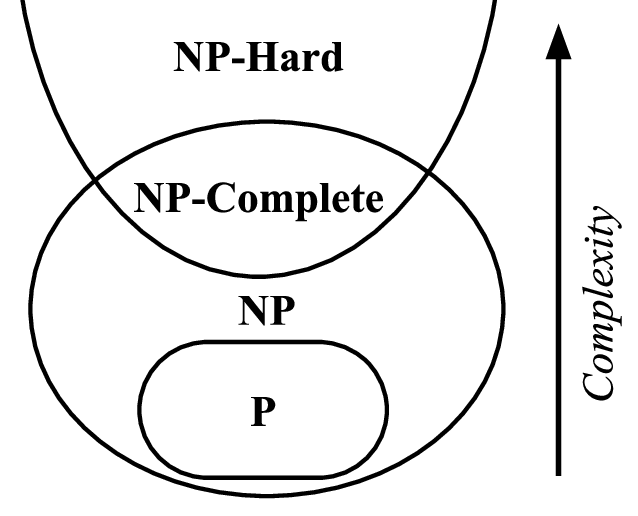
\includegraphics[width = 0.7\textwidth]{images/NP.png}
   \end{frame}

   \begin{frame}{How to solve Combinatorial optimization problem}
     \Large
     \begin{spacing}{1.5}
       \begin{itemize}
         \item Branch and bound
         \item Cutting plane
         \item Column generation
         \item ......
       \end{itemize}
     \end{spacing}
   \end{frame}


   \begin{frame}{Summary}
     Finally, we should master how to settle a problem in that way, so that we will have more ideas and try different methods.

     In the process of practice,they can guarantee to find the global solution, but in solving some typical practical problems, the price is too high, or it is easy to fall into local optimum. Because it's hard to accelerate the algorithm that can guarantee to find the optimal solution, that is, for most practical problems, it is difficult to find polynomial algorithm, because most of them are NP hard problems, then the rest selection is to design an algorithm that can jump out of local optimum.
   \end{frame}


    \section{General Optimization problem}

    \frame{\sectionpage}

    \begin{frame}{Convex Optimization}
      \begin{itemize}
        \only<1>{\item Linear Optimization
        \item Non-Linear Optimization}
        \only<2>{\item Convex Optimization
        \item Non-Convex Optimization}
      \end{itemize}
    \end{frame}

    \begin{frame}{Convex Optimization}
      \begin{itemize}
        \item Convex set
        \item Convex function
        \item Convex optimization problem
      \end{itemize}
      \begin{equation*}
        \begin{align}
        \min &\quad f\end{align}(x) \\
        \text{s.t.} &\quad g_i(x) \leq 0, i=1,2,...,m \\
          &\quad h_j(x) = 0, j = 1,2,...,n
        \end{align}
      \end{equation*}
    \end{frame}

    \begin{frame}{Standard Problem}
      \begin{itemize}
        \item Linear Programming(LP)
        \[
        \begin{aligned}
        \min &\quad c^Tx+d \\
        s.t. &\quad G(x) \preceq h \\
            &\quad A(x) = b
        \end{aligned}
        \]
        \item Quadratic Programming(QP)
        \[
        \begin{aligned}
        \min &\quad \frac{1}{2}x^TPx+c^Tx+d \\
        s.t. &\quad G(x) \preceq h \\
             &\quad A(x) = b
        \end{aligned}
        \]
        \item Semidefinite Programming(SDP)
        \[
        \begin{aligned}
        \min &\quad tr(CX) \\
        s.t. &\quad tr(A_iX)=b_i, i=1,2,....p \\
             &\quad X \succeq 0
        \end{aligned}
        \]
        \item Cone Programming(CP)
      \end{itemize}
    \end{frame}

    \begin{frame}{Other problems}
      \begin{itemize}
        \item Least squares
        \item SVM
        \item QCCP
        \item SOCP
        \item GP
      \end{itemize}
    \end{frame}

    \begin{frame}{Property}
      \begin{itemize}
        \item Local = globle
        \item Non \to Convex
        \item Many method to solve and wide application.
      \end{itemize}
    \end{frame}

    \begin{frame}{Methods}
      \begin{itemize}
        \item Gradient
        Describe the basic iteration process.$x_{k+1}=x_k+\alpha_k d_k$
        $\triangledown f(x_k)^Td_k < 0$
        $f(x_{k+1}) = f(x_k+\alpha_k d_k) < f(x_k)$
        \item Sub-gradient(for can't derivative)
        \item Interior point
      \end{itemize}
    \end{frame}

    \begin{frame}{Gradient}
      Two essential elements: step and gradient. All kinds of methods are based on the fundamental.
      \begin{itemize}
        \item Random
        \item Batch
        \item ......
      \end{itemize}
      convergence condition
    \end{frame}

\begin{frame}{KKT}
  \begin{itemize}
    \item Interior Methods
    \item Penelty
    \item Dual
    \item Lagrange
  \end{itemize}
\end{frame}

\begin{frame}{Non-Convex}
  \item convert to Convex
  \item heuristics
  The important thing is how to jump out of the local optimization.
  Change the parameter by experience.
\end{frame}

\begin{frame}{Random optimization}
  \item Methods
  \item Algorithmic idea
\end{frame}


    \section*{Summary} %You can remove this if you do not want to use it
        \begin{frame}{Summary}
            The author is extremely thankful to Prof. Liu for the short, yet wonderful, conversations about this seminar.
        \end{frame}

    % \section*{References} %You can remove this if you do not want to use it
    %     \nocite{Djairo} \nocite{PhilPanof} \nocite{Fleming} \nocite{Shankar}
    %     \begin{frame}{References}
    %         \printbibliography
    %     \end{frame}

    \section{}
    \begin{frame}{}
        \centering
            \Huge\bfseries
        \textcolor{orange}{The End}
    \end{frame}
\end{document}
